\section{Triển khai hệ thống}
Hiện nay có rất nhiều cách để triển khai của hệ thống phần mềm cho người dùng, sau đây là một số cách triển khai:
\begin{enumerate}
    \item Tự triển khai server: đây là cách thủ công nhất để triển khai ứng dụng web, lập trình viên sẽ cài đặt các công cụ như web server (Apache, Nginx, IIS,...), database server (MySQL, PostgreSQL,...) và triển khai ứng dụng lên server của mình. Phương pháp này đòi hỏi kiến thức về quản trị hệ thống và bảo mật, tuy nhiên nó cung cấp cho lập trình viên sự linh hoạt cao để tuỳ chỉnh và điều khiển ứng dụng của mình.
    \item Platform-as-a-service (PaaS): Đây là phương pháp triển khai ứng dụng web trên một nền tảng được quản lý bởi một nhà cung cấp dịch vụ. Lập trình viên chỉ cần đưa mã nguồn của ứng dụng lên nền tảng PaaS và các công cụ và hạ tầng sẽ được quản lý bởi nhà cung cấp dịch vụ. Các ví dụ về PaaS và Heroku, Google App Engine, Microsoft Azure, Amazon Web Services.
    \item Infrastructure-as-a-service (IaaS): Đây là phương pháp triển khai ứng dụng web trên một hạ tầng đám mây được cung cấp bởi một nhà cung cấp dịch vụ. Lập trình viên có thể tự cấu hình môi trường của mình trên hạ tầng đám mây, bao gồm cả máy chủ ảo, lưu trữ, mạng và các công cụ khác. Các ví dụ về IaaS là Amazon Web Services, Google Cloud Platform và Microsoft Azure.
    \item Docker containers: Đây là phương pháp triển khai ứng dụng web trên các container Docker. Docker cho phép lập trình viên đóng gói ứng dụng và các phụ thuộc của nó trong một container, và triển khai các container này trên bất kỳ máy chủ nào. Phương pháp này đảm bảo tính di động và tương thích với mọi môi trường.
\end{enumerate}
Sau khi cân nhắc thì chúng tôi đã chọn cách tiếp cận là sử dụng PaaS để khiển khai ứng dụng. Đây là một số ưu điểm của các tiếp cận này: 
\begin{enumerate}
    \item Tiết kiệm thời gian và chi phí: Không cần phải chi một khoản tiền lớn cho việc xây dựng, cài đặt phần cứng hay chi phí phát sinh trong khi hệ thống tạm ngừng hoạt động, và không phải tốn thời gian để thiết lập cũng như bảo trì phần lõi.
    \item Tăng tốc độ phát triển: Thiết lập và triển khai đơn giản, nhanh chóng đưa ứng dụng lên giai đoạn production.
    \item Mở rộng dễ dàng: Có thể mở rộng thêm về khả năng lưu trữ cũng như khả năng xử lý khi cần.
    \item Tính linh hoạt cao: cho phép các nhà phát triển có thể tham gia và làm việc trên các ứng dụng ở bất cứ nơi đâu.
\end{enumerate}
Tuy nhiên, PaaS cũng có một số hạn chế, như:
\begin{enumerate}
    \item Phụ thuộc vào nhà cung cấp dịch vụ: việc triển khai hệ thống trên các nền tảng này sẽ phụ thuộc khá nhiều vào khả năng của nhà cung cấp dịch vụ, chẳng hạn như băng thông, dung lượng,... Chỉ có thể chọn lựa những giải pháp có sẵn mà khó lòng tự điều chỉnh theo ý muốn và nhu cầu của nhà phát triển.
    \item Nguy cơ về bảo mật: Mặc dù các nhà cung cấp dịch vụ luôn cố gắng nâng cao và phát triển việc bảo mật nền tảng và cơ sở hạ tầng, vấn đề bảo mật của ứng dụng lại phụ thuộc khá nhiều vào mức độ bảo mật của nền tảng đó.
\end{enumerate}

\subsection{Triển khai phần Frontend của hệ thống}
\subsection{Triển khai phần Backend của hệ thống}
Việc triển khai ở phía backend của ứng dụng sử dụng nền tảng Render như sau:
\newline
Sau khi hoàn tất việc tạo tài khoản hoặc đăng nhập vào Render, chúng ta sẽ tạo một Web Service ở trên nền tảng này:
\begin{figure}[H]
    \centering
    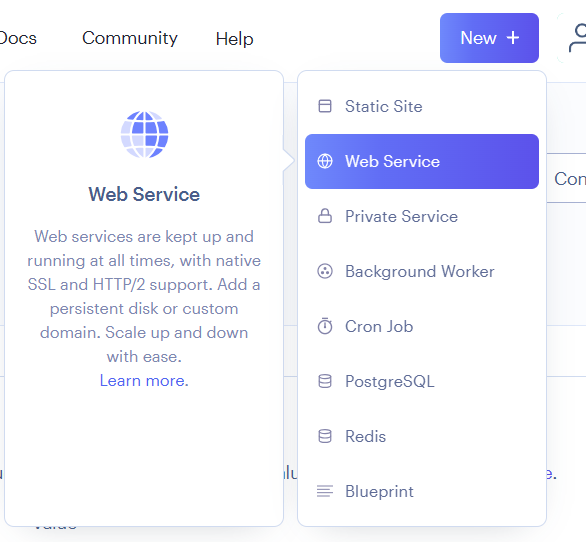
\includegraphics[width=\linewidth]{Content/Hiện thực hệ thống/images/Webservice.png}
    \caption{Giao diện tạo Web service trên Render}
    \label{fig:Tạo Web service}
\end{figure}
Sau đó, ta thiết lập kết nối giữa service trên Render với nơi chứa source code. Ở đây, Render cung cấp 2 lựa chọn là kết nối với Repository trên Github hoặc một Image trên các nền tảng khác. Nhóm chúng tôi lựa chọn phương án đầu tiên.
\begin{figure}[H]
    \centering
    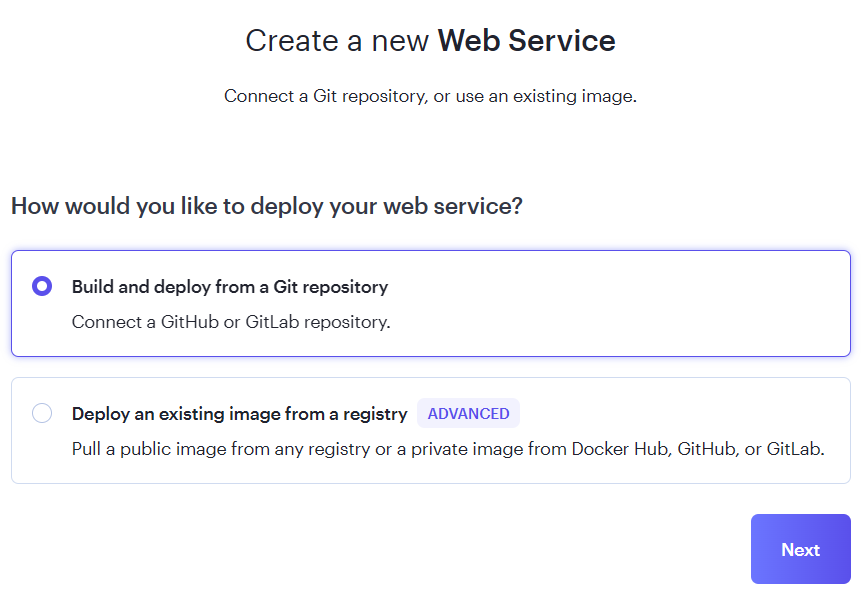
\includegraphics[width=\linewidth]{Content/Hiện thực hệ thống/images/gitrepo.png}
    \caption{Chọn kết nối với Repository}
    \label{fig:Chọn kết nối với Repository}
\end{figure}
Sau đó, chúng ta sẽ chọn kết nối đến một Repository cụ thể. Ở đây, chúng tôi chọn kết nối đến Repository BPE - be tương ứng với phần backend của hệ thống:
\begin{figure}[H]
    \centering
    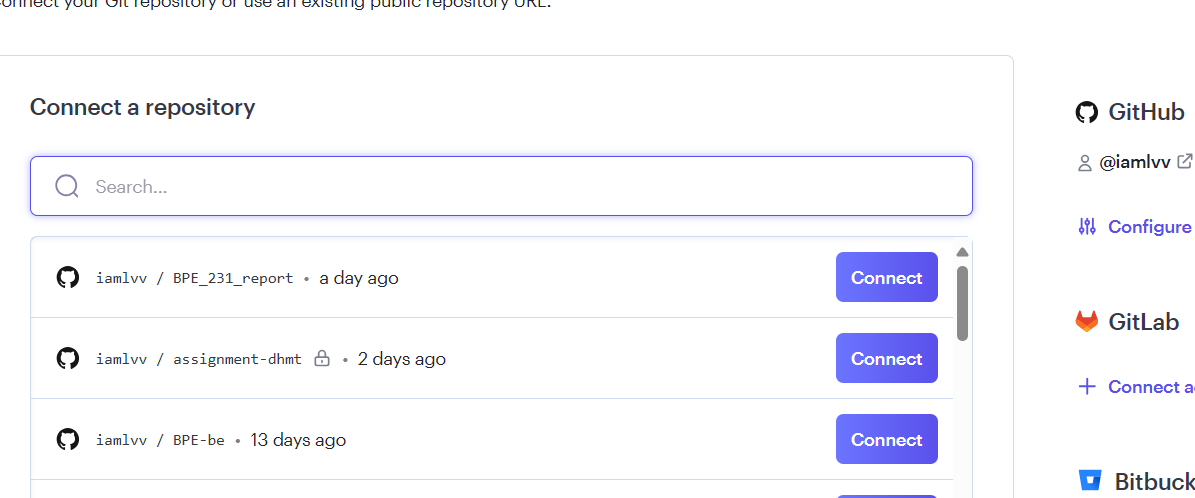
\includegraphics[width=\linewidth]{Content/Hiện thực hệ thống/images/chooserepo.png}
    \caption{Kết nối với Repository của Backend}
    \label{fig:Kết nối với Repository của Backend}
\end{figure}
Sau đó, chúng ta cần điều chỉnh một số những thiết lập để service có thể tự triển khai trên source code của mình. Cụ thể, ta cần chọn nơi đặt server để chạy web service, hay nhánh (branch) trên repository được chọn để triển khai, thiết lập các biến môi trường cũng như câu lệnh để cài đặt các dependencies và khởi chạy server.
\begin{figure}[H]
    \centering
    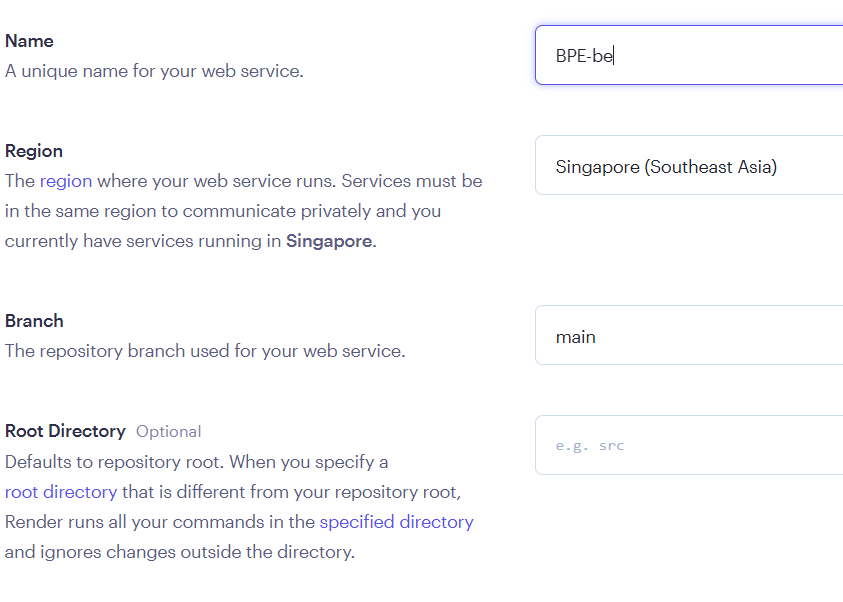
\includegraphics[width=\linewidth]{Content/Hiện thực hệ thống/images/config.png}
    \caption{Thiết lập service}
    \label{fig:Thiết lập service}
\end{figure}
Render cũng cung cấp thêm một số những phiên bản trả phí. Với nhu cầu của chúng tôi đó là một máy chủ luôn trong trạng thái sẵn sàng cho các yêu cầu từ người dùng, và có khả năng lưu trữ file lâu dài, chúng tôi chọn sử dụng phiên bản trả phí Starter - đáp ứng được những nhu cầu trên.
\newline
Như vậy, chúng tôi đã triển khai phần backend của hệ thống lên một PaaS là Render với url \url{https://bpe.onrender.com}. Sau khi triển khai, chúng tôi có thể theo dõi những yêu cầu từ người dùng, cũng như những độ đo khác của hệ thống như băng thông, mức sử dụng CPU, RAM và một số những trạng thái khác.


\subsection{Triển khai phần Database của hệ thống}
Việc triển khai cơ sở dữ liệu của hệ thống được thực hiện trên nền tảng Neon.tech.
Sau khi hoàn tất việc tạo tài khoản hoặc đăng nhập vào Neon.tech, chúng ta sẽ tạo một Database ở trên nền tảng này:
\begin{figure}[H]
    \centering
    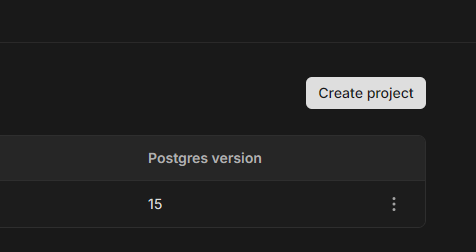
\includegraphics[width=0.5\linewidth]{Content/Hiện thực hệ thống/images/createProjectDB.png}
    \vspace{0.5cm}
    \caption{Giao diện tạo Database trên Neon.tech}
    \label{fig:Tạo Database}
\end{figure}
Sau đó, ta sẽ điều chỉnh một số thông tin về database, chẳng hạn như tên, server lưu trữ:
\begin{figure}[H]
    \centering
    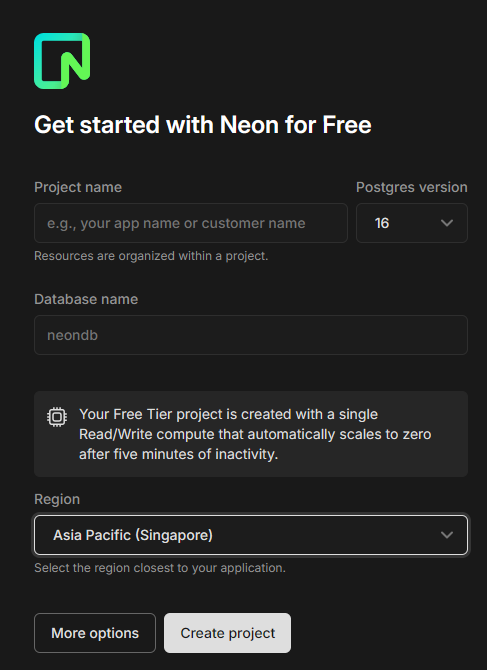
\includegraphics[width=0.5\linewidth]{Content/Hiện thực hệ thống/images/projectDBinfo.png}
    \vspace{0.5cm}
    \caption{Điều chỉnh thông tin Database trên Neon.tech}
    \label{fig:Điều chỉnh thông tin Database}
\end{figure}
Cuối cùng, việc tạo database đã hoàn tất. Neon.tech sẽ tạo ra đường dẫn để ta có thể kết nối tới database này. Ngoài ra,
Neon.tech còn hỗ trợ viết câu lệnh truy vấn, giúp ta có thể thao tác với database một cách dễ dàng.
\begin{figure}[H]
    \centering
    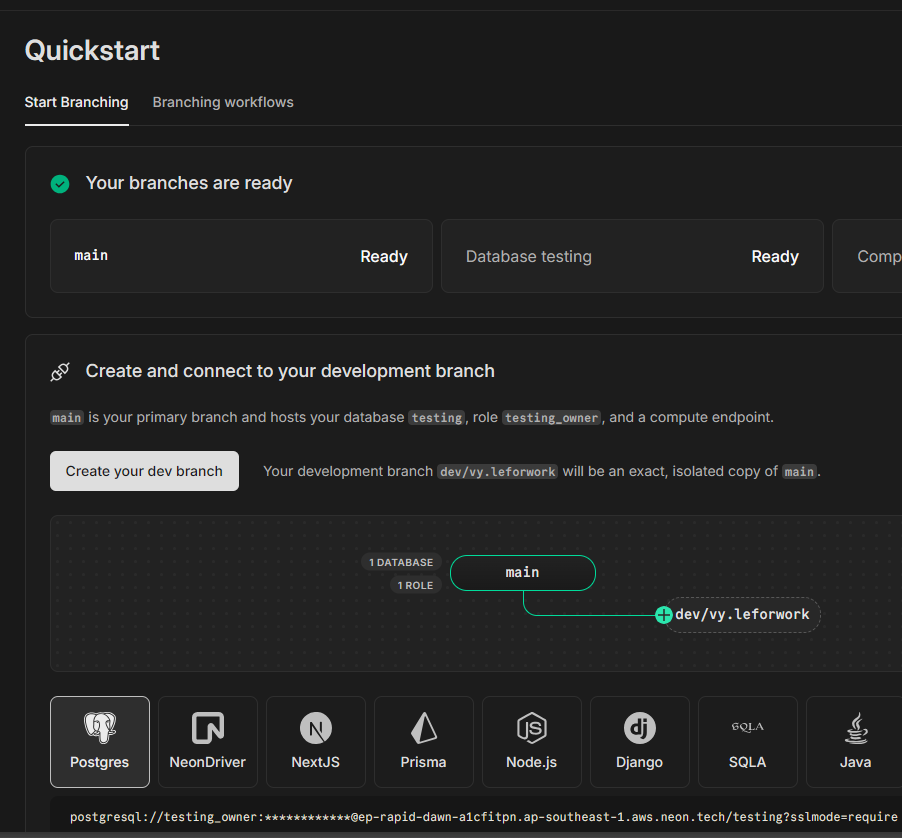
\includegraphics[width=0.5\linewidth]{Content/Hiện thực hệ thống/images/finishDBcreate.png}
    \vspace{0.5cm}
    \caption{Khởi tạo Database thành công}
    \label{fig:Khởi tạo Database thành công}
\end{figure}
